\chapter{Slice sampler}

Los métodos de simulación slice sampler consisten en generar una cadena de Markov que converja a la distribución que se desea muestrear. La idea intuitiva de estos métodos consiste en suponer que el vector aleatorio bivariado $(X,Y)$ se distribuye uniforme en la región que está por debajo de la función de densidad, de la cual obtendríamos una muestra $(X_{0},Y_{0})$, y de está solo nos quedariamos con $X_{0}$, siendo esta nuestra variable de interés.\\ 

Ahora, para generar una muestra uniforme en dicha región, se utiliza un algoritmo recursivo con el fin de tener una cadena de markov que converja a la muestra deseada.\\

En términos ilustrativos el procedimiento es como sigue:\\

$1)$ Supongamos que tenemos el kernel o una densidad de una variable aleatoria univarada $X$, de la cual nos interesaría obtener una muestra aleatoria, y que además la gráfica de esta densidad es de la siguiente manera, por ejemlo:

\begin{figure}[h]
	\centering
	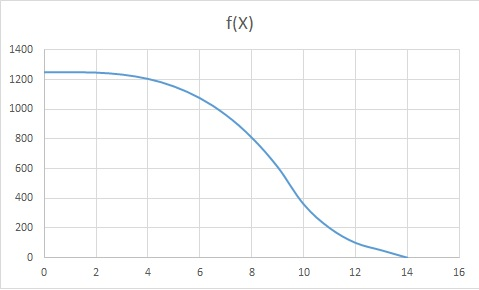
\includegraphics[width=0.7\linewidth]{Figuras/Slicesampler1}
	\caption{}
	\label{Grafica}
\end{figure}

\bigskip
$2)$ Luego definimos el vector aleatorio bivariado $(X,Y)$, el cual suponemos que se distribuye uniforme en la región que está por debajo de la gráfica anterior, y a esta región la denotamos como $U$, por lo que $U$ sería el conjunto de parejas $(x,y)$ con la propiedad de que $x$ es menor a $y$, siendo $y=f(x)$.\\ Entonces la región de la cual nos interesa obtener una muestra se ve de la siguiente forma:

\begin{figure}[h]
	\centering
	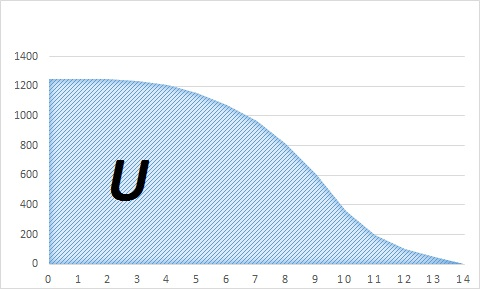
\includegraphics[width=0.7\linewidth]{Figuras/gs2}
	\caption{}
	\label{fig:gs2}
\end{figure}

\bigskip
$3)$ Ahora, proponemos un valor inicial $x_{0}$, y por el anexo (algo), si un vector aleatorio bivariado se distribuye uniforme en alguna región, entonces para cada valor que tome la variable $X$, la distribución marginal de $Y$ dado $X=x_{0}$ se distribuye uniforme dentro del segmento de recta $L(y)=((y,x_{0}) | y\in R)$, donde $L(y)$ está dentro de $U$. De esta manera, podríamos generar una realización de $Y$ dado $x_{0}$, así obtendríamos algún valor $y_{0}$, después fijamos éste valor $y_{0}$, y tendríamos ahora que $X$ dado $y_{0}$ se distribuye uniforme en $U\cap  L(x)=((x,y_{0})|x\in R)$, así obtendríamos una realización de $X$ dado $y_{0}$ de donde obtenríamos nuevamente un valor $x_{0}$. Así repetiriamos el proceso, pues de esta manera tenemos una cadena de Markov que converge a la realización de haber obtenido una muestra uniforme sobre $U$, donde sólo nos interesa el valor de $X$.\\
En la siguiente gráfica se ilustra el punto $3)$, por simplicidad se supuso que el primer valor que tomó la variable $X$ fue 0, luego $Y$ dado $x$ igual a cero se distribuye uniforme en el intervalo $(0,1200)$, de donde ahora obtenemos una realización de $Y$ dado $x$ igual a cero, donde Y tomó ahora el valor de $500$, con esta nueva información actualizamos el valor de $Y$, por lo que ahora obtenemos una realización de $X$ dado $Y$ igual a 500, y así seguimos actualizando los valores de $X$ y $Y$ hasta obtener la muestra deseada.

\begin{figure}[h]
	\centering
	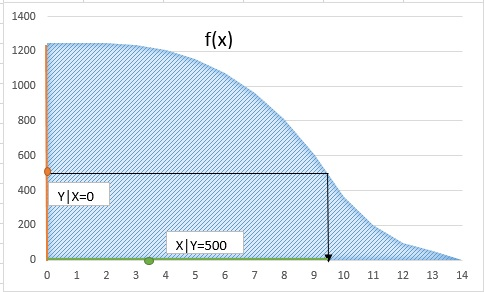
\includegraphics[width=0.7\linewidth]{Figuras/gs3}
	\caption{}
	\label{fig:gs3}
\end{figure}

